\documentclass[a4paper]{article}
\usepackage{graphicx}

\begin{document}

\title{Homework Submission Servlet Working Specification}
\author{Mike Burns}
\date{\today}

\maketitle

Revision 6.

\section{Overview}\label{sec:overview}

The homework submission servlet is a tool for students to electronically submit
homework assignments. It supports username and password authentication,
changing passwords, logging out, account creation, and courses, a separation of
students from non-students, partnerships, assignments, and file submission.
Future goals are task assignment, and online grading.

\section{Use Cases}\label{sec:usecases}

The servlet currently supports users logging in with a valid username and
password, changing their password, selecting a course, adding a partner if
possible, viewing assignments, submitting homework, and logging out. They can
also create an account if they have not already done so.

\subsection{Supported Use Cases}\label{subsec:detailed-usecases}

\begin{itemize}
\item{A user enters an invalid username and/or password pair.}
\item{A user logs in, then logs out.}
\item{A user logs in, then closes the Web browser.}
\item{A user logs in, logs out, uses the back button once, then logs out again.}
\item{A user logs in, sucessfully changes his or her password, then logs out.}
\item{A user logs in, attempts to change his or her password, enters an invalid
old password, then logs out.}
\item{A user logs in, attempts to change his or her password, enters an invalid
old password, sucessfully enters the correct data and changes his or her password,
then logs out.}
\item{A user logs in, attempts to change his or her password, enters mismatched
new passwords, then logs out.}
\item{A user logs in, attempts to change his or her password, enters mismatched
new passwords, sucessfully enters the correct data and changes his or her password,
then logs out.}
\item{A user logs in, selects a course in which he or she is a student, goes to
  the partnership page, adds a partner, logs out.}
\item{A user logs in, selects a course in which he or she is a student, goes to
  the partnership page, sees existing partners, logs out.}
\item{A user logs in, selects a course in which he or she is a student, has a
  partner, views the assignments page, submits a homework, logs out.}
\item{The Web server is restarted by the TA or instructor.}
\end{itemize}

\subsubsection{New Use Cases}\label{subsubsec:newusecases}
\begin{itemize}
\item{A user logs in, selects a course in which he or she is a student, has a
  partner, views the assignments page, submits a homework, logs out.}
\end{itemize}

\section{Goals}\label{sec:goals}

The feature goals of this iteration are:

\begin{itemize}
\item{Homework submission.}
\end{itemize}

\section{Architecture}\label{sec:arch}

The high-level view of the components is described, followed by a breakdown of
the modules and units that are composed to make the servlet.

\subsection{High-Level Components}\label{subsec:high-level}

\begin{figure}[ht]
\centering
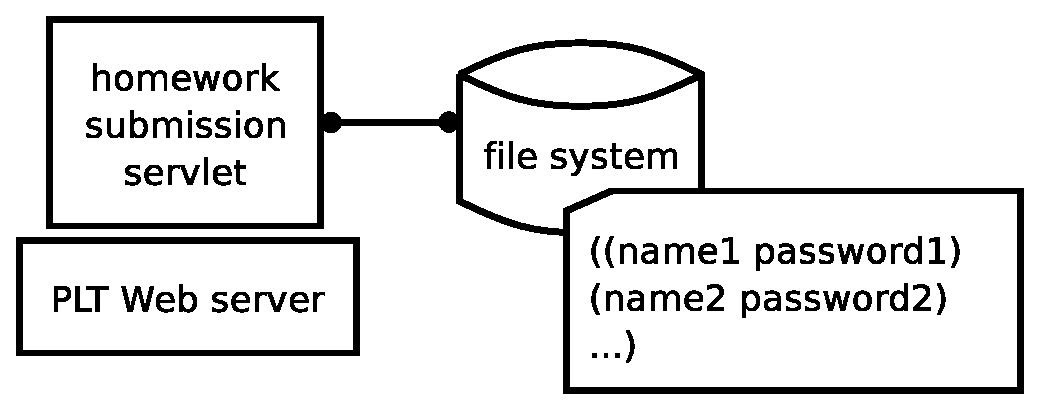
\includegraphics[scale=.35]{architecture.eps}
\caption{High-level view of the homework submission servlet}
\label{fig:architecture}
\end{figure}

The homework submission servlet is a module run by the PLT Web server. The
servlet is a composition of other modules ($\S$\ref{subsec:components}). A
PostgreSQL database with a table holding data about people is connected to the
servlet via the spgsql library.

\subsection{Modules and Units}\label{subsec:components}

At its core, the servlet is a form-based application. The code for generating 
forms and the code for generating transitions between forms are separated into 
separate modules, named pages, and transitions, respecitively.

\begin{figure}[ht]
\centering
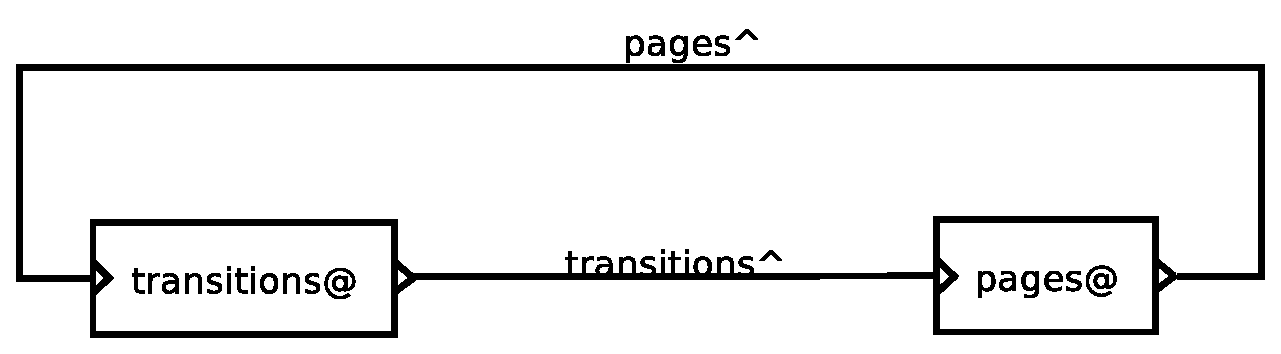
\includegraphics[scale=.30]{units.eps}
\caption{Pages and transitions are mutually recursive}
\label{fig:layout}
\end{figure}

Each page function embeds calls to multiple transitions, and each transition
calls a page function. Because of this recursive dependency, pages and 
transitions are grouped into signed units.

The scheduler module is \verb|requir|ed from both the servlet and the
transitions module. The body of the scheduler module is only executed when the
servlet is first loaded by the Web server, and not when the transitions module
is required by the pages-transitions module.

\subsubsection{Pages-transitions}\label{subsubsec:pages-transitions}

The module \verb|pages-transitions| links and provides the procedures which
create XML ($\S$\ref{subsubsec:pages}) with the procedures that control the
interaction and drive the backend ($\S$\ref{subsubsec:transitions}).

\subsubsection{Pages}\label{subsubsec:pages}

A page is an XML expression (xexpression) with embedded callbacks. These callbacks
are transitions ($\S$\ref{subsubsec:transitions}). Page functions take an
optional xexpression to use as a status message. Pages are defined in the
\verb|pages@| signed unit.

Pages have the form:

\begin{verbatim}
(define page-foo 
 (page (...)
  "Foo"
  ... (hyperlink (transition-bar ...) "Bar") ...))
\end{verbatim}

\paragraph{Interface}\label{para:pages-interface}

The functions provided from the \verb|pages^| signature are as follow. A
\verb|(page? c ...)| is \verb|((c ...) (xexpr?) . opt-> . xexpr/callback?)|.

\begin{verbatim}
page-login : (page?)
\end{verbatim}
Prompt the user for his or her username and password.

\begin{verbatim}
page-student-main: (page? session?)
\end{verbatim}
Confirm the user has logged in as a student.

\begin{verbatim}
page-non-student-main: (page? session?)
\end{verbatim}
Confirm the user has logged in as a non-student.

\begin{verbatim}
page-change-password : (page? session?)
\end{verbatim}
Prompt the user for a new password.

\begin{verbatim}
page-create-user : (page?)
\end{verbatim}
Prompt the user for all the information needed to create a
new account. This is: their name as we know it, the last
four digits of their Northeastern ID, their desired username,
and their password twice.

\begin{verbatim}
page-courses : (page? session? (listof course?))
\end{verbatim}
Show the user all courses he or she is in, allowing him or her to select one.

\begin{verbatim}
page-student-partners : (page? session? (listof String))
\end{verbatim}
The partnerships to which the user belongs, and the ability to add a partner if
the course partnership size allows it.

\begin{verbatim}
page-student-assignments : (page? session? (listof assignment?))
\end{verbatim}
The assignments which the student either has due or had due.

\subsubsection{Transitions}\label{subsubsec:transitions}

A transition is a procedure used to move between pages. There are two categories
of transitions. An action transition performs some backend work
($\S$\ref{subsubsec:backend})---such as updating a password field in the
database---then sends a page to the user. A direct transition sends a page to
the user without backend work. Transitions are defined in the
\verb|transitions@| signed unit.

Direct transition procedures have the form:

\begin{verbatim}
(define-transition (transition-foo ...)
  (send/suspend/callback (page-foo ...)))
\end{verbatim}

Action transition procedures have the form:

\begin{verbatim}
(define-action-transition (transition-action ...)
  (binding ...)
  (schedule (lambda () (backend-action ...)))
  (send/suspend/callback (page-foo ...)))
\end{verbatim}

\paragraph{Interface}\label{para:transitions-interface}

The procedures provided from the \verb|transitions^| signature are as follow.
A \verb|transition?| is \verb|(request? . -> . xexpr/callback?)|.

\begin{verbatim}
transition-login : transition?
\end{verbatim}
Direct transition to the login page.

\begin{verbatim}
transition-log-out : transition?
\end{verbatim}
Direct transition to the login page. This clears the previously-
stored continuations first through \verb|send/forward|.

\begin{verbatim}
transition-change-password : (session? . -> . transition?)
\end{verbatim}
Direct transition to the change-password page.

\begin{verbatim}
transition-create-user : transition?
\end{verbatim}
Direct transtion to the user creation page.

\begin{verbatim}
transition-courses : (session? . -> . transition?)
\end{verbatim}
Direct transition to the courses selection page.

\begin{verbatim}
transition-student-main : (session? . -> . transition?)
\end{verbatim}
Direct transition to the main page for a student.

\begin{verbatim}
transition-non-student-main : (session? . -> . transition?)
\end{verbatim}
Direct transition to the main page for a non-student.

\begin{verbatim}
transition-student-partners : (session? . -> . transition?)
\end{verbatim}
Direct transition to the partnership management page for students.

\begin{verbatim}
transition-student-assignments : (session? . -> transition?)
\end{verbatim}
Direct transition to the student assignments page.

\begin{verbatim}
transition-view-description : (string? symbol? . -> . transition?)
\end{verbatim}
Direct transition to the description for an assignment.

\begin{verbatim}
transition-log-in : transition?
\end{verbatim}
Action transition to the logged-in page.
Action: Check that the username and password pair are correct.
If the username and password do not match, send page-login with a message.
Otherwise, send page-courses.

\begin{verbatim}
transition-update-password : (session? . -> . transition?)
\end{verbatim}
Action transition to the change-password page.
Action: Change the password.
Send the main page with a message explaining whether changing the password
worked and, if it failed, why.

\begin{verbatim}
transition-create-a-user : transition?
\end{verbatim}
Action transition to the logged-in page.
Action: Create a user with a username and password.
Check the Northeastern ID against the name in the list of
ID/name pairs; if they match, check the passwords; if they
match, and the username is not taken, and the user is not
already created, then create the account and transition to
the main page. Otherwise, transition to the user
creation page with an error explaining which step failed.

\begin{verbatim}
transition-add-partner : (session? . -> . transition?)
\end{verbatim}
Action transition to the partnership management page.
Action: Add a student to the partnership for this student, if legal.
Check that this student is not in a partnership of the correct size for the
course, and that the selected partner entered the correct password. Add
the selected partner to the partnership for this student. Send the partnership
management page.

\begin{verbatim}
transition-submit-assignment : (number? session? . -> . transition?)
\end{verbatim}
Action transition to the assignments page.
Action: upload the homework and store it in the database.
If the student can submit an assignment, store the file on the filesystem and
update the database. Send the assignments page.

\subsubsection{Scheduler}\label{subsubsec:scheduler}

The scheduler is used to solve synchonization problems between servlet threads.
Servlets are run in multiple threads to support multiple users; however, each
thread must access the single database as a shared resource, creating a
synchonization requirement. The database management system uses transactions to
maintain invariants in case of failure, but only takes care of simple
concurrency problems, such as simultaneous access to a table.

A possible solution to this problem is a semaphore; however, semaphores cause
problems with the PLT Web server. Semaphores interact poorly with the timeouts
maintained by the Web server, as demonstrated in the following scenerio (figure
\ref{fig:semaphores}):

\begin{enumerate}
\item{The servlet grabs a semaphore.}
\item{The Web server's timer goes off.}
\item{The Web server's timer kills the servlet, which never has a chance to
post to the semaphore. This locks the servlet until it is manually refreshed.}
\end{enumerate}


%% TODO: Document the timer interactions in the Web server documentation.
%% Include the semaphore problem and the channel solution.

\begin{figure}[ht]
\centering
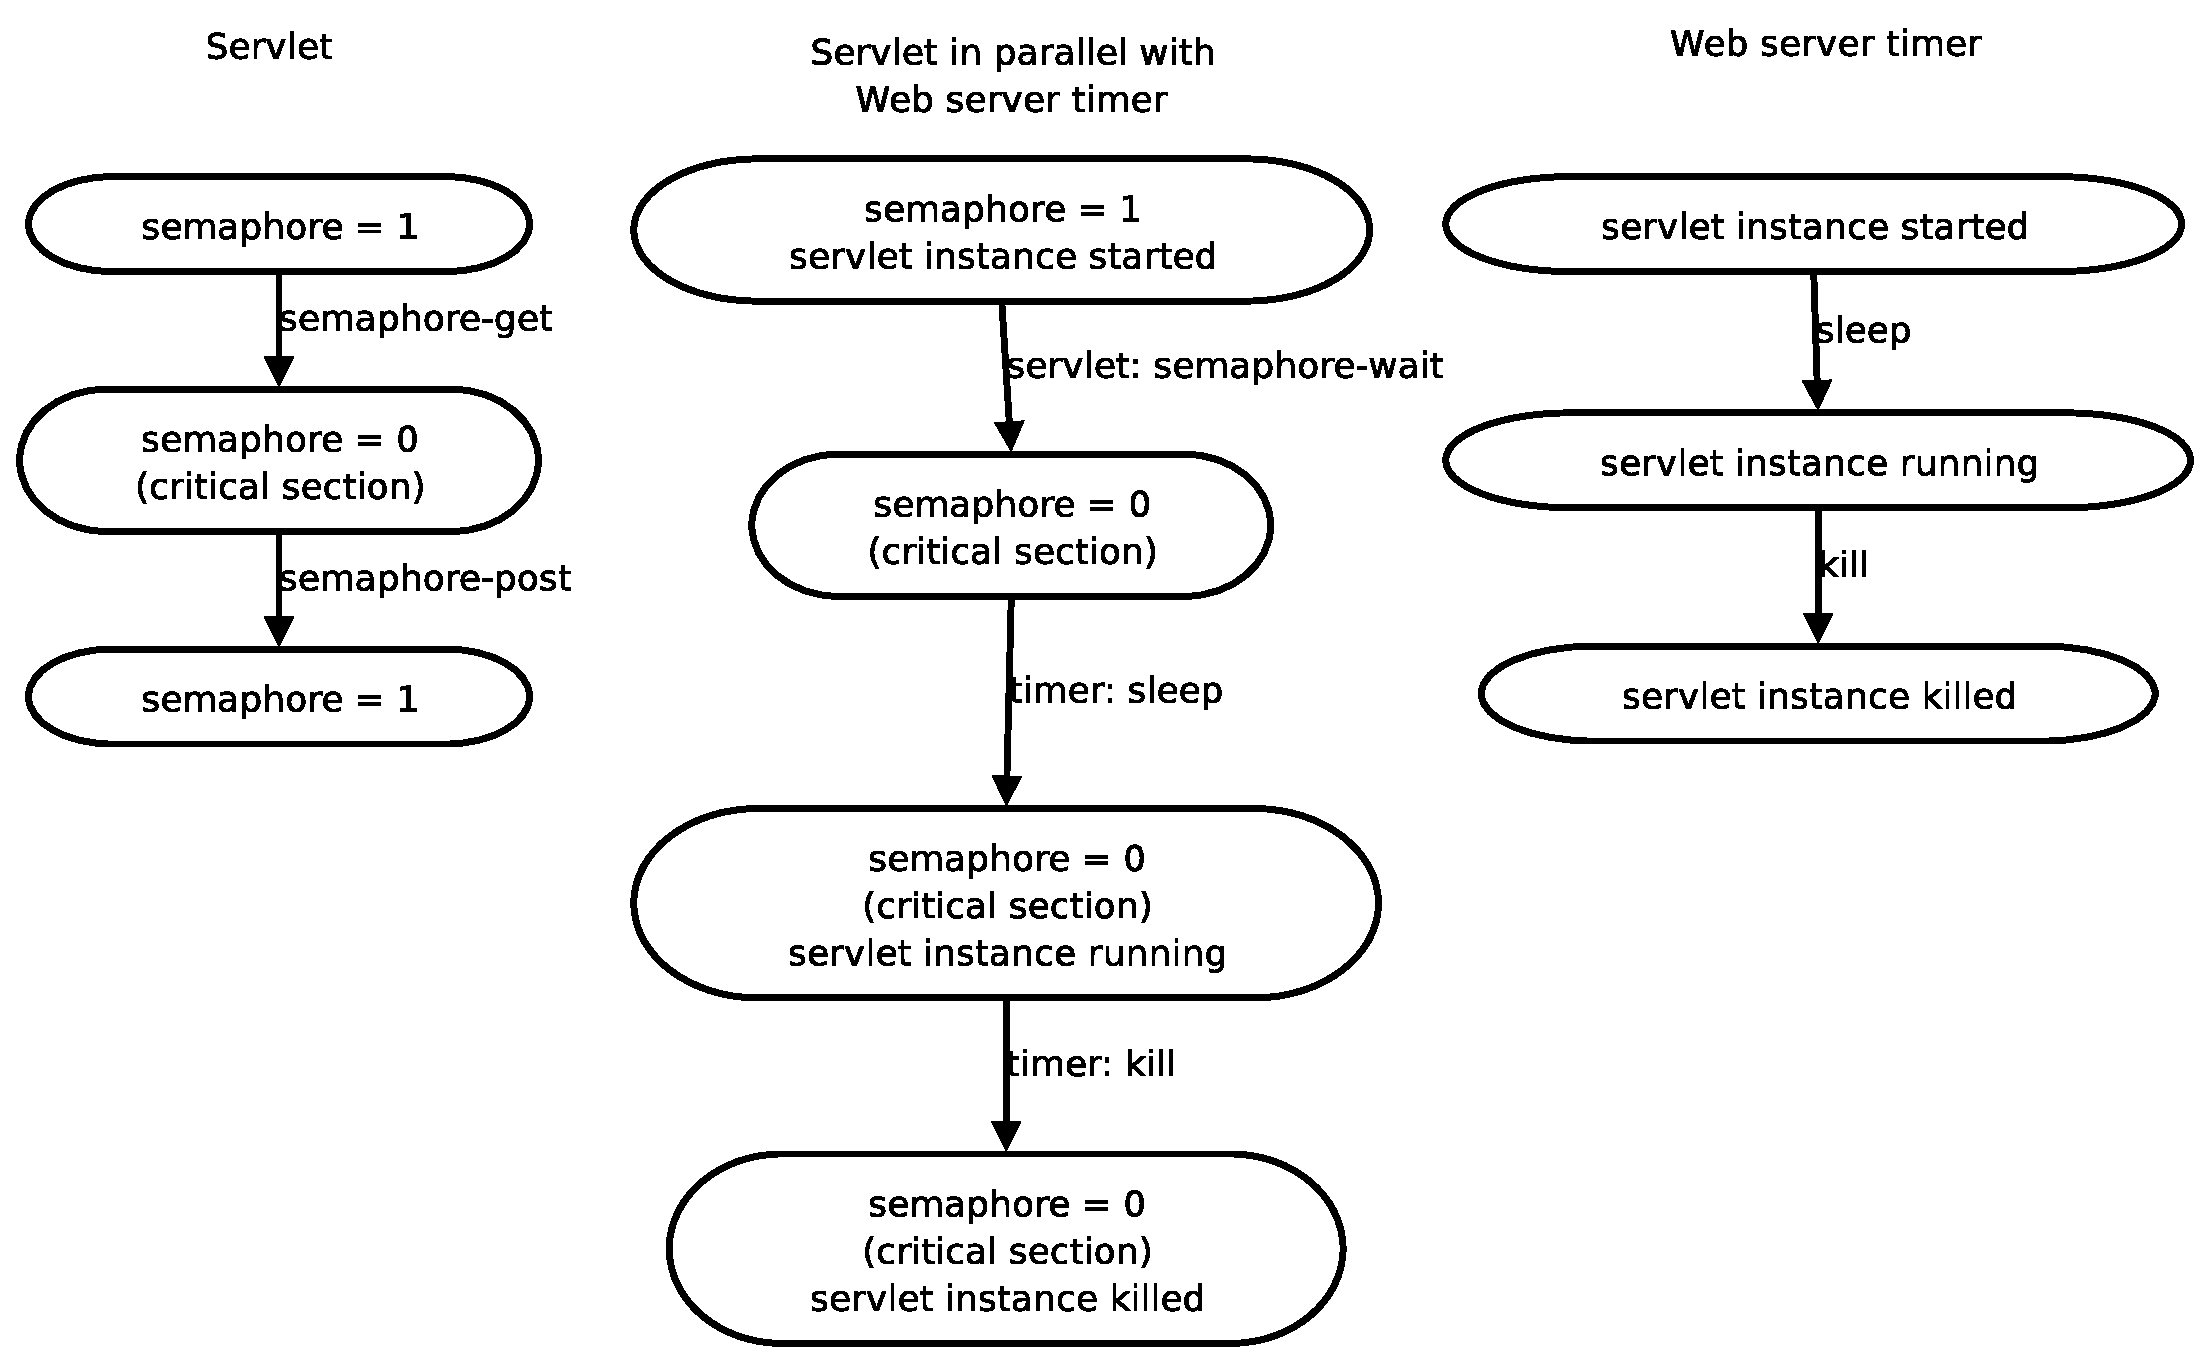
\includegraphics[scale=.30]{semaphore-deadlock.eps}
\caption{Semaphore deadlocking with the timer}
\label{fig:semaphores}
\end{figure}

Instead of semaphores, we use a scheduler based on channels. The scheduler
thread is started before the servlet enters the start state. This thread
performs all procedures that use the shared resource (the database), to
guarantee sequential access to this resource.

\begin{figure}[ht]
\centering
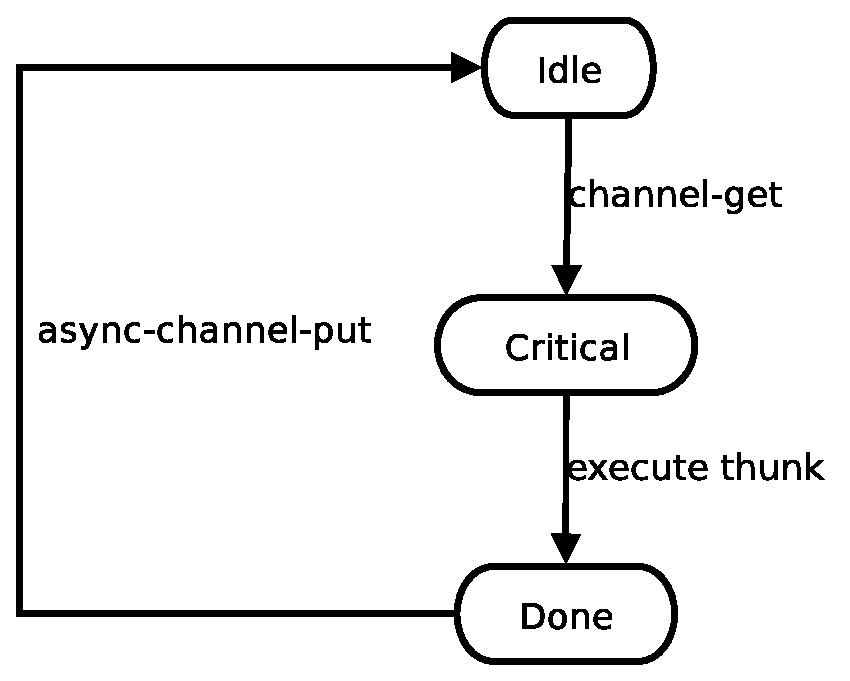
\includegraphics[scale=.30]{channel.eps}
\caption{State diagram of the scheduler based on channels}
\label{fig:channel}
\end{figure}

The thread is a loop that listens on a synchronous channel for requests. A
request must contain a result channel; this result channel is asynchronous so
the scheduler never blocks on a client.

The Web server's timer does not kill this thread because it is started before
the servlet enters the starting state. 

The \verb|schedule| form creates an asynchronous result channel and puts it and
the thunk on the scheduling channel. The result of the \verb|schedule| form is
read from the result channel.

%\begin{figure}[ht]
%\centering
%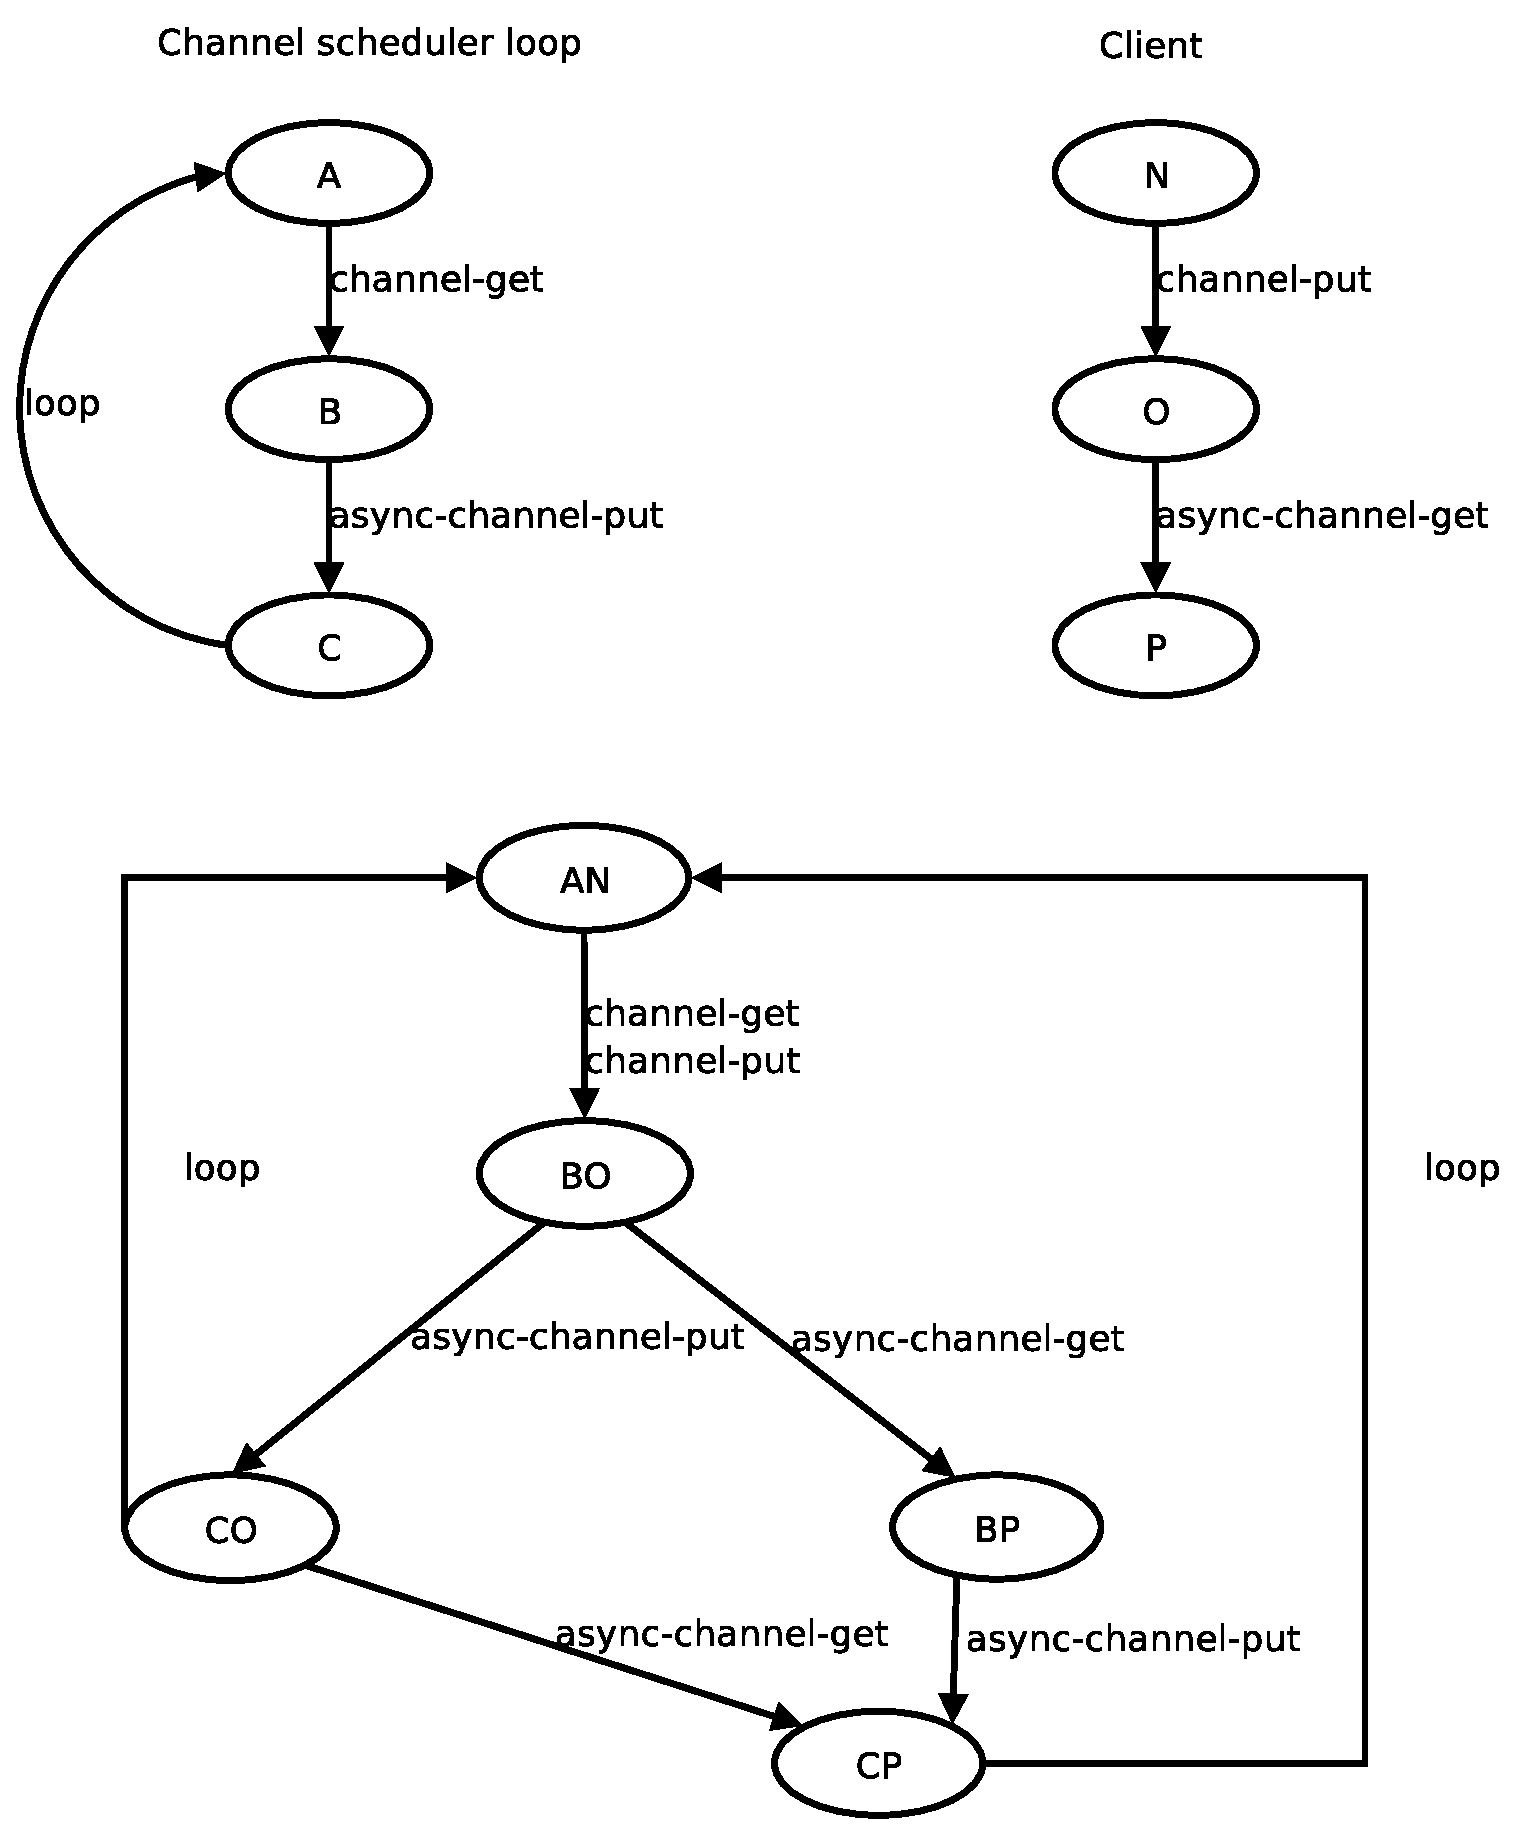
\includegraphics[scale=.30]{kripke-channels.eps}
%\caption{Kripke diagram of the scheduler based on channels with a client}
%\label{fig:kripke-channel}
%\end{figure}

\subsubsection{Backend}\label{subsubsec:backend}

Backend procedures affect the database by selecting data from, inserting data
into, or updating data in the database. The backend module provides procedures
only used by the procedures defined in the \verb|transitions@| signed unit.

The backend uses the PostgreSQL object-relational database management system.
This is a full ACID database using standard SQL92; we use a system of this
complexity to more easily achieve future goals:

\begin{itemize}
\item{Multiple courses.}
\item{Support multiple user roles (e.g. instructor for one course, student in
another).}
\item{Relationships between users (e.g. partnerships, student-grader).}
\end{itemize}

\section{Testing}\label{sec:tests}

Two kinds of tests are run on the homework submission servlet: use case tests
and stress tests. Use case tests are automated tests that verify that the
servlet performs all the specified use cases
($\S$\ref{subsec:detailed-usecases}), with tests for user error. These are
automated using a simulated Web server ($\S$\ref{subsec:use-case-tests}).
Stress tests verify that the servlet and Web server can handle the desired
number of users concurrently and over long periods, without exhausting memory
and other resources.  These are automated by sending requests to the Web server
using HTTP ($\S$\ref{subsec:stresstests}).

\subsection{Use Case Tests}\label{subsec:use-case-tests}

The simulated server framework uses existing Web server modules to create its
own server which then drives the servlet.

\begin{figure}[ht]
\centering
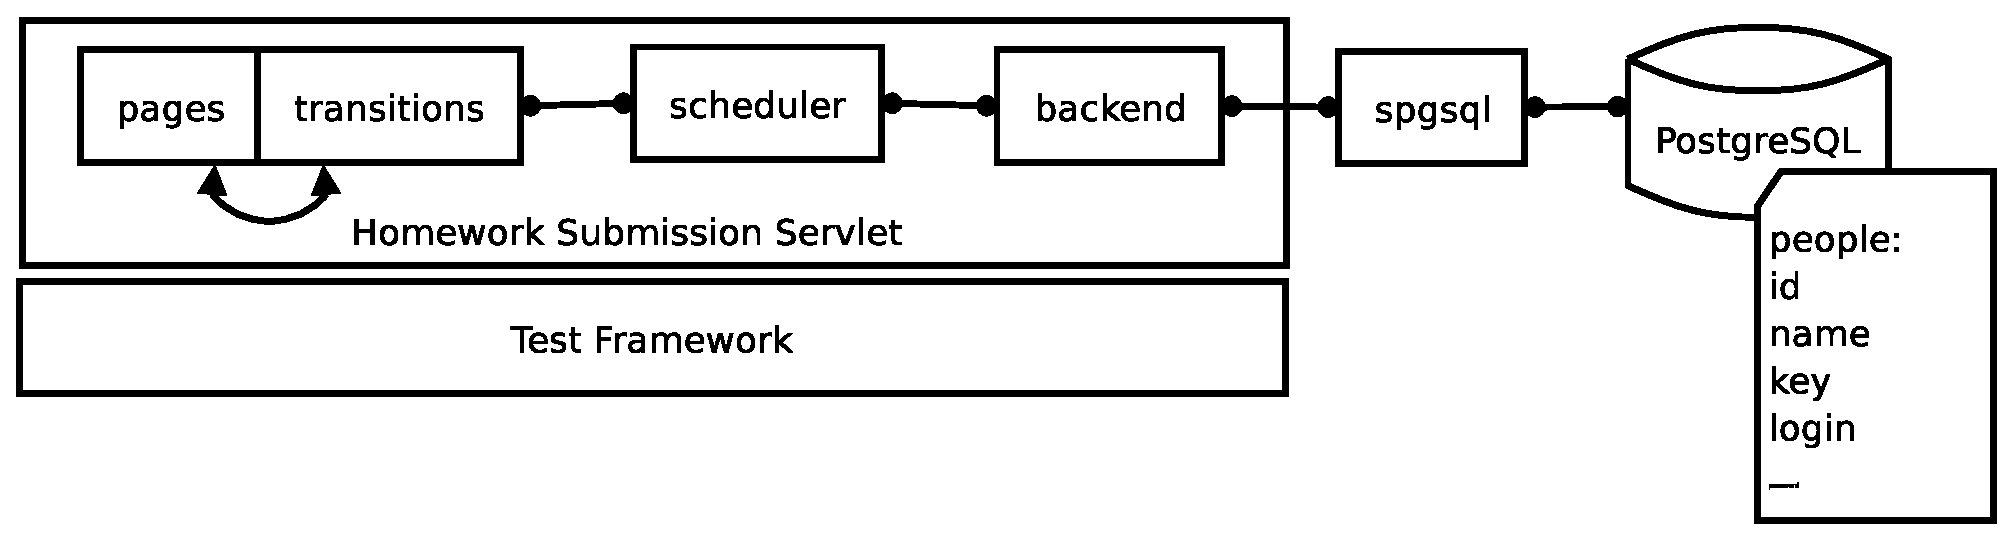
\includegraphics[scale=.30]{servlet-test.eps}
\caption{The servlet test framework replaces the Web server}
\label{fig:servlet-tests}
\end{figure}

%%% 1. Clean up interface for framework
%%% 2. Document
%%% 3. Replace this with a reference to the documentation from (2).

The following tests must pass, using the simulated server framework, as a
student and non-student:

\begin{itemize}
\item{A user enters an invalid username and/or password.}
\item{A user logs in, then logs out.}
\item{A user logs in, then closes the Web browser.}
\item{A user logs in, logs out, goes back to the logged-in page, and logs out
  again.}
\item{A user logs in, sucessfully changes his or her password, then logs out.}
\item{A user logs in, attempts to change his or her password, enters an invalid
  old password, then enters mismatched new passwords, then sucessfully changes
  his or her password, then logs out.}
\item{A user attempts to create an account, enters the wrong Northeastern ID,
  then enters a taken username, then enters mismatched passwords, then succeeds
  in creating an account, then logs out.}
\item{A user logs in, selects a course in which he or she is a student, goes
  to the partnership management page, adds a partner, logs out.}
\item{A user logs in, selects a course in which he or she is a student, goes
  to the partnership management page, views the existing partners, logs out.}
\item{A user logs in, selects a course in which he or she is a student, creates
  a partnership, views assignments, submits an assignment, views its contents,
  logs out.}
\end{itemize}

%%% Note yet done. Not sure how best to do this, either.
In addition, the script to start and stop the Web server must work for all TAs
and instructors.

\subsection{Stress Tests}\label{subsec:stresstests}

The stress-test suite drives the servlet using HTTP 1.0, simulating a real Web
browser hitting the real Web server. Stress tests demonstrate potential
problems this servlet has in a real-life situation.

\begin{figure}[ht]
\centering
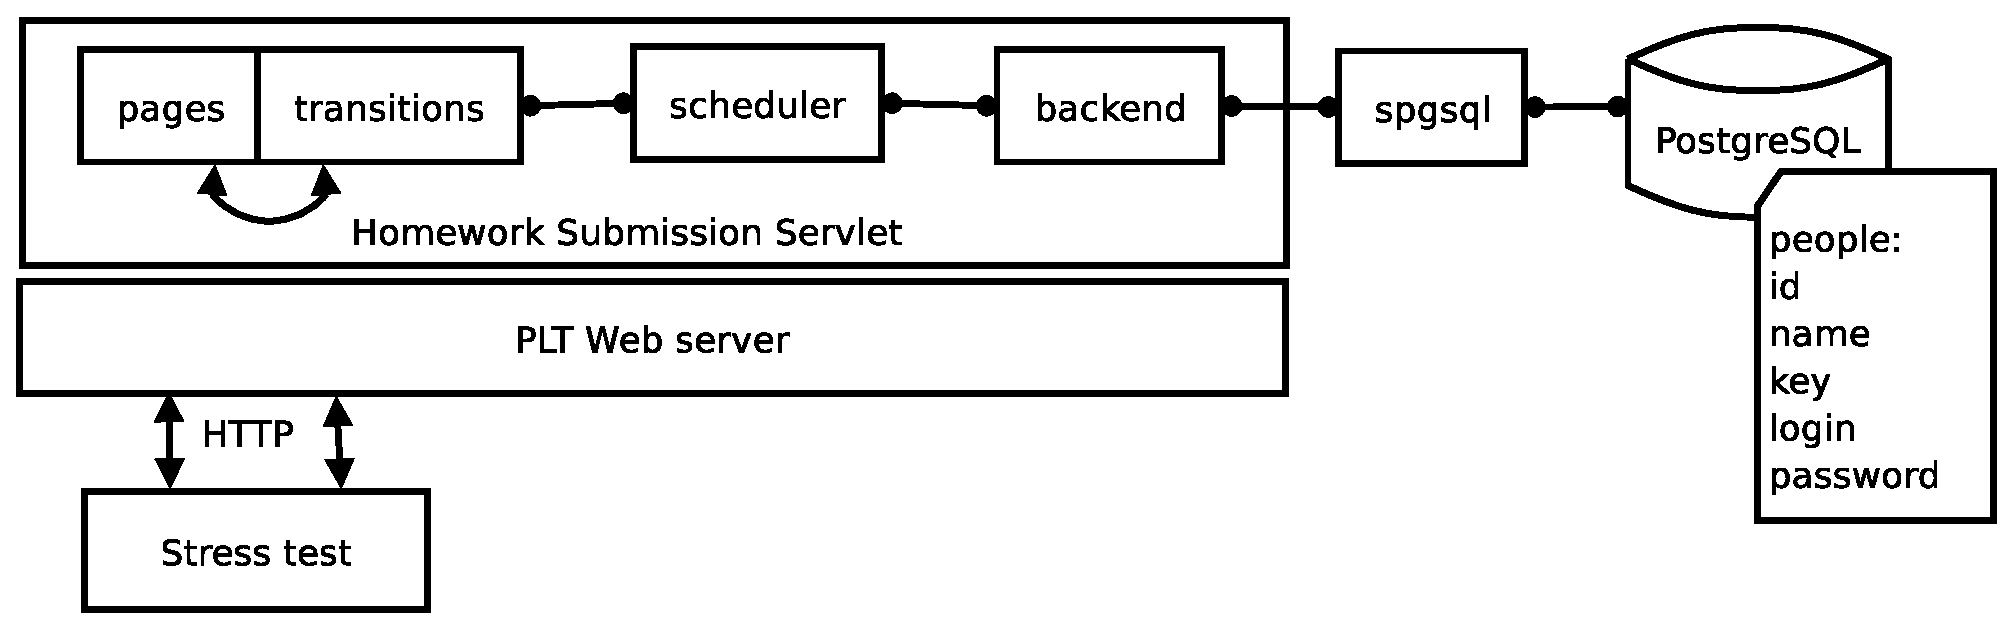
\includegraphics[scale=.30]{stress-test.eps}
\caption{Stress tests use the full Web server via TCP/IP}
\label{fig:stress-tests}
\end{figure}

\subsubsection{Memory Stress}\label{subsubsec:mem-stress}

These tests are run in an unbounded loop, in an attempt to show any memory
leaks and high memory usage in places where the servlet can not clean up after
itself. This simulates how the servlet and server perform over the desired
period of use.

The memory tests are:

\begin{itemize}
\item{A user logs in, then closes the Web browser.}
\end{itemize}

\subsubsection{Concurrency Tests}\label{subsubsec:parrallel-stress}

These tests are to determine how the servlet and server perform during very
heavy, parallel-access load. For this, 1000 concurrent test clients are run
1000 times.

The concurrency tests are:

\begin{itemize}
\item{A user logs in, changes his or her password, then logs out.}
\item{A user logs in, selects a course in which he or she is a student, views
  the assignments page, submits an assignment, logs out.}
%\item{Test the scheduler against timeouts.}
\end{itemize}

%An hourly automated test will be run against the live servlet; if this test
%fails, an email notification will be sent and the Web server restarted.

\section{Documentation}\label{sec:docs}

The documentation provided with this servlet are this outline and three
documents each describing typical use cases for instructors, teaching
assistants, and students, respectively.

\end{document}
